\documentclass[english,10pt, compress]{beamer}
%\documentclass[english,10pt, compress, handout]{beamer}
\usepackage{mathptmx}
\usepackage[T1]{fontenc}
\usepackage[latin9]{inputenc}
\usepackage{color}
\usepackage{array}
\usepackage{multirow}
\usepackage{amsmath}
\usepackage{amssymb}
\usepackage{fancyvrb}
\makeatletter

%%%%%%%%%%%%%%%%%%%%%%%%%%%%%% LyX specific LaTeX commands.
\newcommand{\noun}[1]{\textsc{#1}}
%% Because html converters don't know tabularnewline
\providecommand{\tabularnewline}{\\}

%%%%%%%%%%%%%%%%%%%%%%%%%%%%%% Textclass specific LaTeX commands.
 % this default might be overridden by plain title style
 \newcommand\makebeamertitle{\frame{\maketitle}}%
 \AtBeginDocument{
   \let\origtableofcontents=\tableofcontents
   \def\tableofcontents{\@ifnextchar[{\origtableofcontents}{\gobbletableofcontents}}
   \def\gobbletableofcontents#1{\origtableofcontents}
 }
 \long\def\lyxframe#1{\@lyxframe#1\@lyxframestop}%
 \def\@lyxframe{\@ifnextchar<{\@@lyxframe}{\@@lyxframe<*>}}%
 \def\@@lyxframe<#1>{\@ifnextchar[{\@@@lyxframe<#1>}{\@@@lyxframe<#1>[]}}
 \def\@@@lyxframe<#1>[{\@ifnextchar<{\@@@@@lyxframe<#1>[}{\@@@@lyxframe<#1>[<*>][}}
 \def\@@@@@lyxframe<#1>[#2]{\@ifnextchar[{\@@@@lyxframe<#1>[#2]}{\@@@@lyxframe<#1>[#2][]}}
 \long\def\@@@@lyxframe<#1>[#2][#3]#4\@lyxframestop#5\lyxframeend{%
   \frame<#1>[#2][#3]{\frametitle{#4}#5}}
 \newenvironment{topcolumns}{\begin{columns}[t]}{\end{columns}}
 \def\lyxframeend{} % In case there is a superfluous frame end


%\setbeamersize{text margin left=.5cm, text margin right=.5cm, text}
% I personally don't think the navigation symbols add anything useful

\hypersetup{colorlinks, urlcolor=blue, linkcolor=magenta}

\usetheme{Warsaw}

\DeclareRobustCommand{\CC}{\hbox{C\hspace{-0.5ex}
                       \protect\raisebox{0.5ex}
                       {\protect\scalebox{0.67}{++}}}}



\newcommand{\Emph}[1]{\textcolor{magenta}{{#1}}}


\usefonttheme{serif}
%\usefonttheme{stillsanserifsmall}
\setbeamercovered{transparent}

\makeatother

\usepackage{babel}
\begin{document}





\title[\CC11]{Modern Software Engineering}


\subtitle {Unit Testing}


\author[Dave Steffen]{Dave~Steffen \\
{\tiny with a lot of help
from the C++ Deities.}}


\titlegraphic{
\includegraphics[scale=0.1]{SciTecLogo.jpeg}}

\makebeamertitle


\AtBeginSubsection[]{

  \frame<beamer>{

    \frametitle{Outline}

    \tableofcontents[currentsection,currentsubsection]

  }

}



%\beamerdefaultoverlayspecification{<+->}


\lyxframeend{}\lyxframe{Outline}

\tableofcontents{}




\lyxframeend{}

%%%%%%%%%%%%%%%%%%%%%%%%%%%%%%%%%%%%%%%%%%%%%%%%%%%%%%%%%%%%%%%%%%%%%%
%%%%%%%%%%%%%%%%    SLIDES     %%%%%%%%%%%%%%%%%%%%%%%%%%%%%%%%%%%%%%%
%%%%%%%%%%%%%%%%%%%%%%%%%%%%%%%%%%%%%%%%%%%%%%%%%%%%%%%%%%%%%%%%%%%%%%




\section{Intro: \CC11}

\lyxframeend{}\subsection[\CC 11]{{\CC 11} high points}


\begin{frame}[fragile,t]
\frametitle{\CC11 : Major Changes}

\begin{itemize}

  \item \textquotedblleft{}\CC11 feels like a new language.\textquotedblright{} --- Bjarne Stroustrup
    \pause{}

  \item \textasciitilde{}10 features pervasively change \CC\ coding
    syle, idioms, and guidance.
    \pause{}
    {\scriptsize
    \begin{enumerate}
    \item \Emph{nullptr}
    \item \Emph{auto}
    \item \Emph{initializer lists}
    \item \Emph{range-based for loop}
    \item smart pointers
    \item lambdas
    \item move semantics
    \item Class support / extensions
    \item atomic operations / threading
    \item enum class
    \end{enumerate}
}
\end{itemize}

%}
%\end{columns}
\end{frame}

\lyxframeend{}


\begin{frame}[fragile]
\frametitle{\CC11 References}
\framesubtitle{E.G., where Dave stole all this material from}
\begin{itemize}
  \item New books to update style, idioms and guidance:
    \begin{itemize}
    \item \noun{What:} T\CC~PL 4th Ed (Stroustrup) now available

    \item \noun{Why and How}: Style (Meyers) -- ``Effective Modern
      \CC'',  2014.

    \item \noun{Thou Shalt}: \CC\ Coding Standards (Sutter \&
    Alexandrescu, 2005) updated by an extensive website \url{https://isocpp.org/faq}.

    \end{itemize}
\end{itemize}
\end{frame}
%% \lyxframeend{}




%% \begin{frame}[fragile,t]
%% \frametitle{\CC\ Standards through the ages}
%% \begin{description}
%% \item[1985]: First Commerical Release, T\CC~PL, 1st Ed
%% \item[1991]: T\CC~PL, 2nd Ed, added templates and exceptions
%% \item[1997]: T\CC~PL, 3rd Ed, introduced ISO standard, added STL
%% \item[1998]: ISO \CC Standard (``\CC 98'')
%% \item[2003]: \CC 03 (``bug fix'' ISO Standard)\par
%% \item[2007]: TR1 (library additions): shared\_ptr, hash tables
%% \item[2011]: \CC 11, major revisions (what we're talking about today)
%% \item[2013]: Complete \CC11 implementations (GCC 4.8, CLANG 3.2)
%% \item[2014]: \CC 14   ``Bug fix'' to \CC11
%% \item[2017]: \CC17 New stuff; complete implementation in GCC 7
%% \item[2020]: \CC20 (?) In progress
%% \end{description}
%% \end{frame}


%% \lyxframeend{}%\lyxframe{\CC11 : Major Changes}








%% \begin{frame}[fragile]
%% \frametitle{\CC11 References}
%% \framesubtitle{E.G., where Dave stole all this material from}

%% \begin{itemize}
%% \item {\bf The} \CC\ Web Page: {\url{http://isocpp.org}}.  Has links to the actual standard document, blogs, etc.
%%       \begin{itemize}
%%       \item The FAQ at {\footnotesize \url{https://isocpp.org/faq}} has a section devoted to \CC11 features.
%%       \end{itemize}
%% \item GoingNative12 and 13: a bunch of \emph{really} good
%%       talks. {\footnotesize \url{http://herbsutter.com/2012/02/08/going-native-sessions-online/}} and
%%       {\footnotesize \url{http://channel9.msdn.com/Events/GoingNative/2013}}
%% \item CppCon (took over for GoingNative in 2014) talks on YouTube.
%% \item Stroustrup's home page and FAQ. {\footnotesize \url{http://www2.research.att.com/~bs}}
%% \item Herb Sutter's Blog and GOTW {\footnotesize \url{http://herbsutter.com/}}
%% \item C++ Next, particularly Dave Abrahams' discusson of move
%% semantics: {\footnotesize \url{http://web.archive.org/web/20140113221447/http://cpp-next.com/archive/2009/08/want-speed-pass-by-value/}}


%% \item GCC \CC11/14/17 support: {\footnotesize \url{https://gcc.gnu.org/projects/cxx-status.html}}


%% \end{itemize}


%% \end{frame}



%% \begin{frame}[fragile]
%% \frametitle{The rest of this talk}
%% \framesubtitle{``Hitting the high points''}

%% \begin{itemize}

%%         \item auto
%%         \item uniform initialization / initializer lists
%%         \item range-based for loops
%%         \item nullptr
%% %        \item Class extensions
%% %        \item lambdas (and sermon on standard containers and algorithms)
%% %        \item move semantics
%% %        \item smart pointers (and sermon on RAII, SESE, etc)
%% \end{itemize}

%% \end{frame}

%%%%%%%%%%%%%%%%%%%%%%%%%%%%%%%%%%%%%%%%%%%%%%%%%%%%%%%%%%%%%%%%%%%%%%%%%%%%%%%%
%%%%%%%%%%%%%%%%%%%%%%%%%%%%%%%%%%%%%%%%%%%%%%%%%%%%%%%%%%%%%%%%%%%%%%%%%%%%%%%%
\section{Notes on ``All Your Tests are Terrible...''}
\begin{frame}[fragile,t]
\frametitle{Properties of good tests}

\begin{itemize}
\item \Emph{Unit tests must be easy to run (one button push).}
\item \Emph{Unit tests must return an unambiguous pass/fail result.}
\item Correctness : it tests what it's supposed to test (and
  nothing else)
\item Readability :
\begin{itemize}
  \item Tests don't have tests, so they \emph{must be correct by inspection}
  \item Should read like a novel: setup, action, conclusion, and a happy ending
\end{itemize}
\item Completeness : tests cover the whole API, and only the API
  \begin{itemize}
  \item including edge cases, \emph{particularly} including edge cases
  \item excluding stuff that isn't under test
  \end{itemize}
\item Demonstrability : best documentation of how to use the API.
\item Resilience : ``the notion that your tests should only fail if the
  thing they were actually intended to demonstrate became false, and
  should fail \emph{for no other reason}''
\item \Emph{Test code is just as important as system code}
\end{itemize}

"Note that we didn't call these rules, we did call them goals of good
tests and I don't know that you can necessarily always get all of
them.''
\end{frame}

%%%%%%%%%%%%%%%%%%%%%%%%%%%%%%%%%%%%%%%%%%%%%%%%%%%%%%%%%%%%%%%%%%%%%%%%%%%%%%%%
%%%%%%%%%%%%%%%%%%%%%%%%%%%%%%%%%%%%%%%%%%%%%%%%%%%%%%%%%%%%%%%%%%%%%%%%%%%%%%%%
\begin{frame}[fragile,t]
\frametitle{WRITE TESTS}
\framesubtitle{$\approx 4:00$}
\begin{itemize}
\item good tests are 100\% better than bad tests
\item even bad tests are 10000\% better than no tests
\end{itemize}

\end{frame}

%%%%%%%%%%%%%%%%%%%%%%%%%%%%%%%%%%%%%%%%%%%%%%%%%%%%%%%%%%%%%%%%%%%%%%%%%%%%%%%%
%%%%%%%%%%%%%%%%%%%%%%%%%%%%%%%%%%%%%%%%%%%%%%%%%%%%%%%%%%%%%%%%%%%%%%%%%%%%%%%%
\begin{frame}[fragile,t]
\frametitle{Mocks}
\framesubtitle{$\approx 7:55$} 
(from Wikipedia)
\begin{itemize}
\item {\bf Mock Objects} are simulated objects that mimic the behavior of real objects in controlled ways. 
\end{itemize}

Technically, a Mock is an object that simulates external components
that are changed by the operation in question.
\vskip 6pt
Things that simulate inputs are technically ``stubs'' or something,
but everyone calls them mocks anyway.
\vskip 6pt
Note: mocks need to be tested just like everything else

\end{frame}

%%%%%%%%%%%%%%%%%%%%%%%%%%%%%%%%%%%%%%%%%%%%%%%%%%%%%%%%%%%%%%%%%%%%%%%%%%%%%%%%
%%%%%%%%%%%%%%%%%%%%%%%%%%%%%%%%%%%%%%%%%%%%%%%%%%%%%%%%%%%%%%%%%%%%%%%%%%%%%%%%
\begin{frame}[fragile,t]
\frametitle{Locality}
\framesubtitle{$\approx 11:50$}
Readability: make it clear to the reader why the result is correct.
\vskip 6pt
This is an example of a more general code smell: \Emph{lack of locality}
\vskip 6pt
\begin{itemize}
\item {\bf Locality}: the ability to understand the code without
  looking elsewhere.
\end{itemize}
\vskip 6pt 
Don't assume the reader knows about the other code, has
read the other code, or is going to go look right now.

\vskip 6pt
\begin{center}
\Emph{Tests don't have tests, so correct-by-inspection is all we have
  to prove our tests are correct.}
\end{center}
\end{frame}

%13:00 test fixtures
%16:30 edge cases, 19 important

%%%%%%%%%%%%%%%%%%%%%%%%%%%%%%%%%%%%%%%%%%%%%%%%%%%%%%%%%%%%%%%%%%%%%%%%%%%%%%%%
%%%%%%%%%%%%%%%%%%%%%%%%%%%%%%%%%%%%%%%%%%%%%%%%%%%%%%%%%%%%%%%%%%%%%%%%%%%%%%%%
\begin{frame}[fragile,t]
\frametitle{Black box tests}
\framesubtitle{$\approx 21:00 - 33:00$}
Definitions:
\begin{itemize}
  \item {\bf Black-box testing:} tests use only the public
    interface of the test article.  (The test article is a ``black box'' you can't see
    inside of.)
  \item {\bf White-box testing:} tests access the internal state of
    the test article. (You can ``see inside the box'').  Also
    ``clear-box'', ``glass-box'', etc.
\end{itemize}
\vskip 6pt
Black box testing is much preferred over white-box, to the degree that
many people say ``Black-box is the only way to test'' and ``White-box
testing is a mistake''.

\vskip 6pt
That's overstating the case.  Black-box is better, but not always
doable. We'll see how to white-box test below,
and discuss the pros and cons.

\end{frame}

%%%%%%%%%%%%%%%%%%%%%%%%%%%%%%%%%%%%%%%%%%%%%%%%%%%%%%%%%%%%%%%%%%%%%%%%%%%%%%%%
%%%%%%%%%%%%%%%%%%%%%%%%%%%%%%%%%%%%%%%%%%%%%%%%%%%%%%%%%%%%%%%%%%%%%%%%%%%%%%%%
\begin{frame}[fragile,t]
\frametitle{Test Result Data}
\framesubtitle{$\approx 29:00$}
Hyrum and Titus make fun of the ``run your code to generate the output
that you verify your code against''.  But...
\begin{itemize}[<+->]
\item We did exactly this on OCEANA as a system test -- run the whole
  thing, get output, save it to a ``canon'' file, compare with that.
\item Note that this does not test that the system is correct, just
  that it hasn't changed.
\item This is \emph{still} really useful when refactoring or
  optimizing.
\item And.... \emph{it found a bug}.  The output didn't compare
  roughly 1/3 times.
\item We had nondeterministic behavior, and who knows how long it
  would have taken us to notice.
\item (Look up ``strict weak ordering'' in sorting predicates)
\end{itemize}
\pause{}
\Emph{Bad tests are still 10000\% better than no tests.}
\end{frame}



%%%%%%%%%%%%%%%%%%%%%%%%%%%%%%%%%%%%%%%%%%%%%%%%%%%%%%%%%%%%%%%%%%%%%%%%%%%%%%%%
%%%%%%%%%%%%%%%%%%%%%%%%%%%%%%%%%%%%%%%%%%%%%%%%%%%%%%%%%%%%%%%%%%%%%%%%%%%%%%%%
\begin{frame}[fragile,t]
\frametitle{Sustainability, and Properties of good tests}
\framesubtitle{$\approx 44:58 - 47:00$}


\begin{itemize}
\item Again: write tests, bad tests are better than no tests
\end{itemize}


\end{frame}

%%%%%%%%%%%%%%%%%%%%%%%%%%%%%%%%%%%%%%%%%%%%%%%%%%%%%%%%%%%%%%%%%%%%%%%%%%%%%%%%
%%%%%%%%%%%%%%%%%%%%%%%%%%%%%%%%%%%%%%%%%%%%%%%%%%%%%%%%%%%%%%%%%%%%%%%%%%%%%%%%
\begin{frame}[fragile,t]
\frametitle{Culture}
\framesubtitle{$\approx 57:25$}
\begin{itemize}
\item Tests are only part of the solution (Defence in depth)
\begin{itemize}
\item code review
\item proper testing
\item static analysis
\item dynamic analysis
\item hardening code
\item canarying
\item production monitoring
\end{itemize}

\item Culture
\end{itemize}


\end{frame}


\section{Engineering and Management Concerns}
%%%%%%%%%%%%%%%%%%%%%%%%%%%%%%%%%%%%%%%%%%%%%%%%%%%%%%%%%%%%%%%%%%%%%%%%%%%%%%%%
%%%%%%%%%%%%%%%%%%%%%%%%%%%%%%%%%%%%%%%%%%%%%%%%%%%%%%%%%%%%%%%%%%%%%%%%%%%%%%%%
\begin{frame}[fragile,t]
\frametitle{Software Engineering Considerations}
Code is hard or impossible to unit test \emph{unless designed with
  this in mind}.
\begin{itemize}
\item Testability is just as important as any other design
  consideration
\item Experience, across the industry and personally, shows that
  designing for testability \emph{improves design}.  (Examples to
  follow).
\item Experience across the industry shows that writing the test
  \emph{before} writing the code improves design.  This is the heart
  of TDD (Test-Driven Development).
\item Black-box testing is always preferred over white-box testing.
\item \Emph{Test code must be treated as system code}.  It's not a
  second-class citizen.
\begin{itemize}
  \item Test code must be as clean, elegant, and maintainable as
    system code.
  \item Test harness, frameworks, and tooling must be designed as
    carefully as anything else
  \item Test code must be code-reviewed just as intently, and held to
    the same high standards, as system code.
  \item \emph{Test code is what lets you sleep soundly at night.
      Treat it accordingly.}
\end{itemize}
\end{itemize}

\end{frame}


%%%%%%%%%%%%%%%%%%%%%%%%%%%%%%%%%%%%%%%%%%%%%%%%%%%%%%%%%%%%%%%%%%%%%%%%%%%%%%%%
%%%%%%%%%%%%%%%%%%%%%%%%%%%%%%%%%%%%%%%%%%%%%%%%%%%%%%%%%%%%%%%%%%%%%%%%%%%%%%%%
\begin{frame}[fragile,t]
\frametitle{Management Considerations}
\begin{itemize}
  \item Testing takes time.
  \item Writing unit tests for exisiting code that
    probably already works is \Emph{incorrectly} considered to be a
    zero-return-on-investment activity.
    \begin{itemize}
      \item ROI might be small but is not
        zero. Consider that without unit tests....
      \item You can't fix bugs in that old code \emph{reliably} 
      \item You can't refactor that old code \emph{reliably}
      \item You can't prove that the code continues to work across
        changes to the code base (or compiler, or deliver OS, or...)
        \item You can not \Emph{provably} maintain your code base without them.
    \end{itemize}
  \item Without unit tests, your code base \emph{is not maintainable}
    without constant activity from superheroes.
\end{itemize}
\end{frame}
%%%%%%%%%%%%%%%%%%%%%%%%%%%%%%%%%%%%%%%%%%%%%%%%%%%%%%%%%%%%%%%%%%%%%%%%%%%%%%%%
%%%%%%%%%%%%%%%%%%%%%%%%%%%%%%%%%%%%%%%%%%%%%%%%%%%%%%%%%%%%%%%%%%%%%%%%%%%%%%%%

\begin{frame}[fragile,t]
\frametitle{Management Considerations}
\framesubtitle{part 2: religion}


Problem: testing takes time, money, schedule, etc. but
prevents problems later.  How do you measure the time / schedule slip
/ budget overrun \emph{that never happens}?  
\vskip 6pt
You can't.
\vskip 6pt

So is this a kind of a religion?  (No, because we have vast amounts of
evidence.)

\begin{itemize}

\item Testing takes a lot of time, in predictable amounts, at predictable
and controllable times.

\item Tracking down mysterious bugs takes unknowable amounts of time,
  at unpredictable moments, usually right before a release.

\end{itemize}

Balancing testing vs budget vs schedule is always hard.  Hold the line.

\end{frame}


%%%%%%%%%%%%%%%%%%%%%%%%%%%%%%%%%%%%%%%%%%%%%%%%%%%%%%%%%%%%%%%%%%%%%%%%%%%%%%%%
%%%%%%%%%%%%%%%%%%%%%%%%%%%%%%%%%%%%%%%%%%%%%%%%%%%%%%%%%%%%%%%%%%%%%%%%%%%%%%%%
%% \begin{frame}[fragile,t]
%% \frametitle{Software Engineering Considerations}
%% \end{frame}

\section{How To Test...}
%%%%%%%%%%%%%%%%%%%%%%%%%%%%%%%%%%%%%%%%%%%%%%%%%%%%%%%%%%%%%%%%%%%%%%%%%%%%%%%%
%%%%%%%%%%%%%%%%%%%%%%%%%%%%%%%%%%%%%%%%%%%%%%%%%%%%%%%%%%%%%%%%%%%%%%%%%%%%%%%%
\subsection{Floating point operations}
\begin{frame}[fragile,t]
\frametitle{Testing Floating Point}
\framesubtitle{}
This may be obvious, but it bears repeating:
{\scriptsize\
\begin{verbatim}
TEST( FloatingTest, division_test) {
  ASSERT_TRUE ( (1.0/3.0) * 3 == 3 );
}
\end{verbatim}}
is a bad idea.  Good frameworks have a set of floating-point
``approximately equals-to'' assertions of the $\Delta < \epsilon$
variety:
{\scriptsize\
\begin{verbatim}
  ASSERT_NEAR( (1.0/3)*3, 3, 1e-14 );
\end{verbatim}}
\begin{itemize}
  \item Consider making adapters for user-defined mathematical types
    (e.g. Vectors) so they are similarly supported by the framework.
  \item Proceed with care!  Consider if ``approximately the same to
    within $\epsilon$'' means
\begin{itemize}
  \item Relative error?
  \item Absolute error?
  \item Units-of-Last-Place (ULP) error?  (used for looking
    specifically at floating-point roundoff).
\end{itemize}
\end{itemize}
Warning: most test frameworks provide OK-but-not-great support for
this.  You may have to roll your own if you're serious about error bounds.
\end{frame}

%%%%%%%%%%%%%%%%%%%%%%%%%%%%%%%%%%%%%%%%%%%%%%%%%%%%%%%%%%%%%%%%%%%%%%%%%%%%%%%%
%%%%%%%%%%%%%%%%%%%%%%%%%%%%%%%%%%%%%%%%%%%%%%%%%%%%%%%%%%%%%%%%%%%%%%%%%%%%%%%%
\subsection{Test for Failure}
\begin{frame}[fragile,t]
\frametitle{Testing Failure Modes}
\framesubtitle{}
It is vitally important to test not just that the code works, but that
it fails the right way.
{\scriptsize\
\begin{verbatim}
int factorial (int n);

TEST( FactorialFunction, Factorial_Failure) {

  ASSERT_THROW( factorial(-1), std::range_error );

  ASSERT_EQ ( factorial (13), -1 );
}
\end{verbatim}}
This test case fails if:
\begin{itemize}
  \item Calling factorial (-1) throws something other than std::range\_error 
  \item Succeeds (doesn't throw anything) 
  \item Calling factorial (13) returns 1932053504 (which is what you get on my laptop after integer overflow -- 
    the answer is 6227020800) rather than -1
\end{itemize}

That is to say, the unit test \emph{fails} if the function \emph{doesn't} fail the right way.  This can be confusing.

\end{frame}


\subsection{Classes with pure virtual functions}
%%%%%%%%%%%%%%%%%%%%%%%%%%%%%%%%%%%%%%%%%%%%%%%%%%%%%%%%%%%%%%%%%%%%%%%%%%%%%%%%
%%%%%%%%%%%%%%%%%%%%%%%%%%%%%%%%%%%%%%%%%%%%%%%%%%%%%%%%%%%%%%%%%%%%%%%%%%%%%%%%
\begin{frame}[fragile,t]
\frametitle{Testing Abstract Base Classes (ABCs)}
\framesubtitle{the problem}
Consider:
{\scriptsize\
\begin{verbatim}
class AbstractBase {
  public:

  virtual int PureVirtual () = 0

  int NonVirtualSquare(int i) {
    return i*i;
  }
};

class Widget : public AbstractBase; // non-abstract
class Wicket : public AbstractBase; // "
\end{verbatim}}
How do I unit test the NonVirtualSquare method?
{\scriptsize\
\begin{verbatim}
\\in AbstractBase_test.cpp

TEST( AbstractBase_test, NVSquareTest {
  AbstractBase i;  // oops! compile error
  ASSERT_EQ( i.square(5), 25 );
}
\end{verbatim}}
\end{frame}
%%%%%%%%%%%%%%%%%%%%%%%%%%%%%%%%%%%%%%%%%%%%%%%%%%%%%%%%%%%%%%%%%%%%%%%%%%%%%%%%
%%%%%%%%%%%%%%%%%%%%%%%%%%%%%%%%%%%%%%%%%%%%%%%%%%%%%%%%%%%%%%%%%%%%%%%%%%%%%%%%
\begin{frame}[fragile,t]
\frametitle{Testing ABC's}
\framesubtitle{the solution?}
You could test in one of the derived classes:
{\scriptsize\
\begin{verbatim}
// in Widget_test.cpp

TEST( WidgetTest, NVSquareTest {
  Widget i;  // ok
  ASSERT_EQ( i.square(5), 25 );
}
\end{verbatim}}
... but a failure shows up in Widget's test suite, not in
AbstractBase's test suite where it belongs.  Widget's test suite
fails, but Widget isn't incorrect.

\end{frame}

%%%%%%%%%%%%%%%%%%%%%%%%%%%%%%%%%%%%%%%%%%%%%%%%%%%%%%%%%%%%%%%%%%%%%%%%%%%%%%%%
%%%%%%%%%%%%%%%%%%%%%%%%%%%%%%%%%%%%%%%%%%%%%%%%%%%%%%%%%%%%%%%%%%%%%%%%%%%%%%%%
\begin{frame}[fragile,t]
\frametitle{Testing ABC's}
\framesubtitle{the solution!}
Instead, derive a test class for the purpose:
{\scriptsize\
\begin{verbatim}
// in AbstractBase_test.cpp  (the AbstractBase's test suite)

class AbstractBaseTester : public AbstractBase {
  virtual int PureVirtual () { ... } // some implementation 
};

TEST( AbstractBaseTest, NVSquareTest {
  AbstractBaseTester i;  // ok
  ASSERT_EQ( i.square(5), 25 );
}
\end{verbatim}}
The tester class is only visible in the unit test, and allows all the
functionality of the abstract base class to be exercised.

\end{frame}


%%%%%%%%%%%%%%%%%%%%%%%%%%%%%%%%%%%%%%%%%%%%%%%%%%%%%%%%%%%%%%%%%%%%%%%%%%%%%%%%
%%%%%%%%%%%%%%%%%%%%%%%%%%%%%%%%%%%%%%%%%%%%%%%%%%%%%%%%%%%%%%%%%%%%%%%%%%%%%%%%
\subsection{Test Classes Not Methods}
\begin{frame}[fragile,t]
\frametitle{Testing Class Behavior}
\framesubtitle{The plot thickens}
This section based on
``Test Smells and Fragrances Kevlin Henney'' 
{\scriptsize\
\begin{verbatim}
class Cup {
  ...
  Cup();            // new cups are empty
  bool IsEmpty(); 
  bool Fill();    // Fills completely, returns false on failure
  bool Drink();   // Empties completely, "
};

\end{verbatim}}

Side note: the interface is interesting, in that:
\begin{itemize}
  \item Filling a full cup is not an error, it's just a failure
    (wastes beer).
  \item Drinking from an empty cup is not an error, it's just
    dissapointing.
\end{itemize}


\end{frame}

%%%%%%%%%%%%%%%%%%%%%%%%%%%%%%%%%%%%%%%%%%%%%%%%%%%%%%%%%%%%%%%%%%%%%%%%%%%%%%%%
%%%%%%%%%%%%%%%%%%%%%%%%%%%%%%%%%%%%%%%%%%%%%%%%%%%%%%%%%%%%%%%%%%%%%%%%%%%%%%%%
\begin{frame}[fragile,t]
\frametitle{Black-box testing conundrum}
``A test suite tests a collection of member functions'' : test each member function separately
{\scriptsize\
\begin{verbatim}
// test the constructor             
TEST( CupTests, constructor) {      
  Cup cup;                      // new cups are supposed to be empty       
  ASSERT_TRUE( cup.IsEmpty() ); // test this.
}                                   

// test IsEmpty                       
TEST( CupTests, testIsEmpty) {        
  Cup cup;                      // empty by construction 
  ASSERT_TRUE( cup.IsEmpty() ); // test ... uh, didn't we just do this?
 }

\end{verbatim}}
Without reaching into the Cup class and examining internal state:
\begin{itemize}
\item we can't verify the constructor's postconditions without a correct
IsEmpty method
\item  and we can't verify the IsEmpty method without a cup
in a known state.
\end{itemize}

\Emph{Is this class untestable?}

\end{frame}

%%%%%%%%%%%%%%%%%%%%%%%%%%%%%%%%%%%%%%%%%%%%%%%%%%%%%%%%%%%%%%%%%%%%%%%%%%%%%%%%
%%%%%%%%%%%%%%%%%%%%%%%%%%%%%%%%%%%%%%%%%%%%%%%%%%%%%%%%%%%%%%%%%%%%%%%%%%%%%%%%
\begin{frame}[fragile,t]
\frametitle{Black-box testing conundrum}
\begin{itemize}[<+->]
\item We could ignore the problem (``Goofus'').
\item Maybe test something else?
{\scriptsize\
\begin{verbatim}
// test IsEmpty                       
TEST( CupTests, testIsEmpty) {        
  Cup cup;

  ASSERT_TRUE( cup.IsEmpty() ); // just to be sure

  cup.Fill(); // should be full

  ASSERT_TRUE( not cup.IsEmpty() );
 }                                     
\end{verbatim}}
\item First... ``just to be sure''?  Do you really expect that to
  fail?  What are you testing? (but people do this a lot)
\item Second... this assumes that Fill works, this is even worse
\end{itemize}
\pause{}
\begin{center}
\Emph{Fundamentally, if we only test via public interface, we eventually
have a circular-logic problem: you have to use the interface to
test the interface, so at some point you have to trust something, right?}
\end{center}
\end{frame}


%%%%%%%%%%%%%%%%%%%%%%%%%%%%%%%%%%%%%%%%%%%%%%%%%%%%%%%%%%%%%%%%%%%%%%%%%%%%%%%%
%%%%%%%%%%%%%%%%%%%%%%%%%%%%%%%%%%%%%%%%%%%%%%%%%%%%%%%%%%%%%%%%%%%%%%%%%%%%%%%%
\begin{frame}[fragile,t]
\frametitle{Test for consistent behavior}
The solution is to \emph{not} take a
member-function-by-member-function approach.  \Emph{Test the class, not the
member functions.}
{\scriptsize\
\begin{verbatim}
TEST( CupTests, A_New_Cup_Is_Empty) {        
  Cup cup;
  ASSERT_TRUE( cup.IsEmpty() ); 
 }                                     

Test( CupTests, An_Empty_Cup_Can_Be_Filled) {
  Cup cup;                   // empty, proved above
  ASSERT_TRUE( cup.Fill() ); // Fill returns true on success
}

TEST( CupTests, A_Filled_Cup_Is_Full) {
  Cup cup;
  cup.Fill();
  ASSERT_TRUE( not cup.IsEmpty() );
}  
\end{verbatim}}

\begin{itemize}
\item Note the vastly improved test names.
\item Testing the class \emph{as a whole}, not individual methods.
\item But have we really broken the circular logic loop?
\end{itemize}
\end{frame}

%%%%%%%%%%%%%%%%%%%%%%%%%%%%%%%%%%%%%%%%%%%%%%%%%%%%%%%%%%%%%%%%%%%%%%%%%%%%%%%%
%%%%%%%%%%%%%%%%%%%%%%%%%%%%%%%%%%%%%%%%%%%%%%%%%%%%%%%%%%%%%%%%%%%%%%%%%%%%%%%%
\begin{frame}[fragile,t]
\frametitle{Test for consistent behavior}

\begin{itemize}
\item Note that we are now testing \emph{consistency of the
  interface}, \Emph{not} \emph{correctness of the implementation}
\item Repeat the previous sentence to yourself several times.
\item This is Popper's falsifiability criterion: you can't prove it
  true, you can just fail to prove it false.
\item \Emph{SCIENCE!}
\end{itemize}

This class exhibits \emph{cohesion}, which is a good thing, and it
means precicely that we can't get ``under its skin'' without surgery.

\begin{center}
\Emph{If a class exhibits correct and consistent behavior in all
  cases, we must declare it correct, even if the implementation is
  nothing but mutually cancelling bugs.}
\end{center}

\end{frame}

%%%%%%%%%%%%%%%%%%%%%%%%%%%%%%%%%%%%%%%%%%%%%%%%%%%%%%%%%%%%%%%%%%%%%%%%%%%%%%%%
%%%%%%%%%%%%%%%%%%%%%%%%%%%%%%%%%%%%%%%%%%%%%%%%%%%%%%%%%%%%%%%%%%%%%%%%%%%%%%%%
\begin{frame}[fragile,t]
\frametitle{Test for consistent behavior}
\framesubtitle{prove it's not correct}
{\scriptsize\
\begin{verbatim}
class Cup {

  Cup() : empty_(false) {}                 // wrong!

  bool IsEmpty() { return not empty_; }      // wrong!

  bool Fill() { 
    if (not empty_) {  // backwards
      empty_ = true;   // backwards
      return true;
    ...
  }
  ...
private:
  bool empty_;
};
\end{verbatim}}
\vskip 6pt
\begin{itemize}
\item This \emph{should not pass code review}, but it is nevertheless
\emph{provably correct}.

\item The implementation is correct, it's just horribly confusing.

\item Black-box testing can't tell the difference, and that's the point.
\end{itemize}
\end{frame}


%%%%%%%%%%%%%%%%%%%%%%%%%%%%%%%%%%%%%%%%%%%%%%%%%%%%%%%%%%%%%%%%%%%%%%%%%%%%%%%%
%%%%%%%%%%%%%%%%%%%%%%%%%%%%%%%%%%%%%%%%%%%%%%%%%%%%%%%%%%%%%%%%%%%%%%%%%%%%%%%%
\subsection{White Box Testing}
\begin{frame}[fragile,t]
\frametitle{White Box Testing}
\framesubtitle {The idea}
Alternately, we could abandon black-box testing.
{\scriptsize\
\begin{verbatim}
// Cup.h                                 // Cup_test.cpp
                                         
class Cup {                              
                                         #include <Cup.h>                    
  Cup() : empty_(true) {}                                                    
                                                                             
  bool IsEmpty() { return empty_; }      TEST( CupTests, TestConstructor)         
                                         {                                        
  bool Fill() {                             Cup c;                                
    if (empty) {                            ASSERT_TRUE( c.empty_ ); // error!
    ...                                  }                           
  }
  ...                                       
private:
  bool empty_;
};
\end{verbatim}}
This won't compile (empty\_ is a private member variable), but if it
did, we would have absolute, unambigous proof that new cups are empty.

How can we make this work?

\end{frame}

%%%%%%%%%%%%%%%%%%%%%%%%%%%%%%%%%%%%%%%%%%%%%%%%%%%%%%%%%%%%%%%%%%%%%%%%%%%%%%%%
%%%%%%%%%%%%%%%%%%%%%%%%%%%%%%%%%%%%%%%%%%%%%%%%%%%%%%%%%%%%%%%%%%%%%%%%%%%%%%%%
\begin{frame}[fragile,t]
\frametitle{White Box Testing}
\framesubtitle {The idea}
This is a horrible idea, but it actually works on most compilers:
{\scriptsize\
\begin{verbatim}
// Cup.h                                 // Cup_test.cpp
                                         #define private public
class Cup {                              
                                         #include <Cup.h>
  Cup() : empty_(true) {}                
                                         
  bool IsEmpty() { return empty_; }      TEST( CupTests, TestConstructor)         
                                         {                                        
  bool Fill() {                             Cup c;                                
    if (empty) {                            ASSERT_TRUE( c.empty_ ); // fine!
    ...                                  }
  }
  ...
private:
  bool empty_;
};
\end{verbatim}}
\begin{itemize}
\item This is, formally, undefined behavior.
\item One undisputed advantage: we can test Cup without changing the code.
\end{itemize}
\begin{center}
\Emph{Don't do this!}
\end{center}
\end{frame}

%%%%%%%%%%%%%%%%%%%%%%%%%%%%%%%%%%%%%%%%%%%%%%%%%%%%%%%%%%%%%%%%%%%%%%%%%%%%%%%%
%%%%%%%%%%%%%%%%%%%%%%%%%%%%%%%%%%%%%%%%%%%%%%%%%%%%%%%%%%%%%%%%%%%%%%%%%%%%%%%%
\begin{frame}[fragile,t]
\frametitle{White Box Testing}
\framesubtitle {The standard solution}
If we are going to break encapsulation, do it correctly
{\scriptsize\
\begin{verbatim}
// Cup.h                                 // Cup_test.cpp
                                         #include <Cup.h>
class Cup {                              
                                         class CupTester {
  Cup() : empty_(true) {}                   bool& empty_;    // proxy 
                                            
  bool IsEmpty() { return empty_; }         CupTester(Cup& c) 
                                              : empty_(c.empty_) {}
  bool Fill() {                           };  
    if (empty) {                         
    ...                                  TEST( CupTests, TestConstructor)     
  }                                      {                                    
                                            Cup c;                            
  friend class CupTester;                   CupTester tester(c);
                                            ASSERT_TRUE( tester.empty_ ); 
};                                        }
\end{verbatim}}
\begin{itemize}
\item Cup declares a tester friend class
\item The friend class exposes Cup's innards
\end{itemize}
This is the recommended way to do white-box testing.
\end{frame}


%%%%%%%%%%%%%%%%%%%%%%%%%%%%%%%%%%%%%%%%%%%%%%%%%%%%%%%%%%%%%%%%%%%%%%%%%%%%%%%%
%%%%%%%%%%%%%%%%%%%%%%%%%%%%%%%%%%%%%%%%%%%%%%%%%%%%%%%%%%%%%%%%%%%%%%%%%%%%%%%%
\begin{frame}[fragile,t]
\frametitle{White-Box Pros and Cons}

Cons:
\begin{itemize}
\item Tests are tightly coupled to implementation.
\begin{itemize}
  \item Changing the implementation breaks the unit tests.
  \item Keeping the unit tests working is an increased maintenance burden.
\end{itemize}
\item Tests no longer document the correct way to use a class
\item Tests can get much more complicated
\item Test authors are no longer bound by the class interface,
  reducing the pressure to improve a bad interface design.
\end{itemize}

Pros:
\begin{itemize}
\item Eash access to internal state makes tests easy to write
\item Requires very minor changes to code
\item Doesn't require redesign or refactoring
\item For some complex cases, it's the only viable option.
\end{itemize}


\end{frame}


%% %%%%%%%%%%%%%%%%%%%%%%%%%%%%%%%%%%%%%%%%%%%%%%%%%%%%%%%%%%%%%%%%%%%%%%%%%%%%%%%%
%% %%%%%%%%%%%%%%%%%%%%%%%%%%%%%%%%%%%%%%%%%%%%%%%%%%%%%%%%%%%%%%%%%%%%%%%%%%%%%%%%
%% \begin{frame}[fragile,t]
%% \frametitle{Software Engineering Considerations}
%% \end{frame}


%% \section[The Problem]{Memory Management Is The Problem}
%% 
\begin{frame}[fragile,t]
\frametitle{Dynamic Memory Is Hard}
\framesubtitle{``If you write C-style code, you expect to have C-style problems'' -- Stroustrup}

{\scriptsize \begin{verbatim}
void foo() {
  double* d = new double[70];
  ...
  if (condition1)
    return;       // Leak!
  ...
  if (error)
    throw ex;     // Leak!

  foo()           // if an exception happens
                  // in here -- Leak!

  delete d;      // cleanup (?)
}
\end{verbatim}}
\end{frame}




%%%%%%%%%%%%%%%%%%%%%%%%%%%%%%%%%%%%%%%%%%%%%%%%%%%%%%%%%%%%%%%%%%%%%%
\begin{frame}[fragile,t]
\frametitle{SESE}

Single-Entry-Single-Exit is an attempt to mitigate this problem:

\begin{columns}[t]
\column{.5\textwidth}
Heavily nested if-blocks:
{\scriptsize\begin{verbatim}
void foo() {
  if (precondition1) {
    double* d = new double[70];
    if (d) {
      ...
      if (precondition2) {
        Widget* w = new Widget;
        if (w) {
           // finally do some work
           FiddleWidget(w);
           ...
           }
        delete w;
        }
     }
   delete d[];
   }
  return;
}
\end{verbatim}}
\pause{}
\column{.5\textwidth}
And doesn't help anyway
{\scriptsize\begin{verbatim}


// Can throw in C++11



// ... might throw



// might throw






\end{verbatim}}
\end{columns}
\pause{}
In the presence of exceptions, \Emph{every function call} can exit the function
\end{frame}


%%%%%%%%%%%%%%%%%%%%%%%%%%%%%%%%%%%%%%%%%%%%%%%%%%%%%%%%%%%%%%%%%%%%%%

\begin{frame}[fragile,t]
\frametitle{Exceptions Break Things}
\framesubtitle{If you don't know what you're doing}
In the presence of exceptions, writing code the old way is nearly impossible:
{\scriptsize\
\begin{verbatim}
void foo() {
  try {  double* d = new double[70]; }
  catch (...) {...}
  ...
  try { foo(); }
  catch (...) { delete d; ...}

  try { bar(); } 
  catch (...) { delete d; ...}

  delete d;      // cleanup
}
\end{verbatim}
}
Every statement must be wrapped in a try/catch block... this is part of the reason exceptions have a bad rap in C++.
\end{frame}

%%%%%%%%%%%%%%%%%%%%%%%%%%%%%%%%%%%%%%%%%%%%%%%%%%%%%%%%%%%%%%%%%%%%%%

\begin{frame}[fragile,t]
\frametitle{}
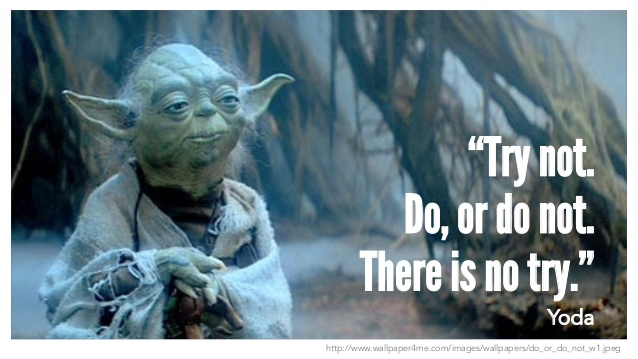
\includegraphics[scale=0.5]{yoda.jpg}

Many (most?) C++ code bases \emph{do not use exceptions}, including
Google's, and including ours.

Writing code \emph{as if} in the presence of exceptions makes code better.

\end{frame}

\begin{frame}[fragile,t]
\frametitle{A Rant}
\framesubtitle{Before we go on...}
There is something very wrong here:
\pause{}
{\scriptsize \begin{verbatim}
void foo() {

  Widget* w = new Widget;
  ...
  if (condition1)
    return;       // Leak!
  ...
  if (error)
    throw ex;     // Leak!

  foo()           // an exception happens
                  // in here -- Leak!

  delete w;      // cleanup 
}
\end{verbatim}}
\pause
\Emph{This isn't Java, so stop it.}

\end{frame}

\begin{frame}[fragile,t]
\frametitle{A Rant}
\framesubtitle{Before we go on...}
Don't hit the heap if you don't have to!

{\scriptsize \begin{verbatim}
void foo() {

  Widget w;      // On the stack!
  ...
  if (condition1)
    return;       // nothing to leak
  ...
  if (error)
    throw ex;     // no problems

  foo()           // an exception happens in here... ok
}
\end{verbatim}}
\pause{}
\begin{itemize}
\item Save runtime
\item Reduce pressure on the heap
\item Reduce memory fragmentation
\pause{}
\item \Emph{Repent, ye Java programmers}
\end{itemize}

\end{frame}

%%%%%%%%%%%%%%%%%%%%%%%%%%%%%%%%%%%%%%%%%%%%%%%%%%%%%%%%%%%%%%%%%%%%%%%%%%%%%%%%

\begin{frame}[fragile,t]
\frametitle{Why dynamic memory at all?}
\center{When must we hit the heap?}
\vskip 6pt
\pause{}

\begin{enumerate}
\item We don't know how many we need until runtime
{\scriptsize \begin{verbatim}
int n;
cin >> n;
Widget* widgets = new Widget[n];
\end{verbatim}
}
\pause{}
\item We don't know what type we need until runtime (polymorphism)
{\scriptsize \begin{verbatim}
class DooDad : public Widget {};
class DooHickey : public DooDad {};
class Gadget : public Widget{}
class Thingy : public Gadget{};

Widget* widget = WidgetFactory(...);
\end{verbatim}
}
\pause{}
\item We don't know how long it's going to live (special case of \#1)
\end{enumerate}

\vskip 12pt
\pause{}

\center{ \Emph{Dynamically allocate only when absolutely necessary} }
\end{frame}


%% \section[The Solution]{The Solution: RAII}
%% %%%%%%%%%%%%%%%%%%%%%%%%%%%%%%%%%%%%%%%%%%%%%%%%%%%%%%%%%%%%%%%%%%%%%%
\begin{frame}[fragile,t]
\frametitle{RAII}
\framesubtitle{Resource Aquisition Is Initialization}
\begin{itemize}
\item Smart pointers are a specific case of a more general idiom, ``RAII''
\item Developed to manage resources in the presence of exceptions, but
  they are much more widely useful.
\item The key idea:  \Emph{Tie resource management to object lifetime}
\item Resource manager objects receive the resource in their
  ctor, and release it in their dtor.  Emphasis:
\begin{itemize}
  \item Allocate resource in constructor (at initialization)
  \item Release resources in destructor (at scope exit)
\end{itemize}
\item Normal scoping rules now ensure proper cleanup.
\item Exceptions cause local variables to be destructed, so no leaks.
\end{itemize}
\vskip 12pt
\pause{}
\center{\Emph{ The most important operation in \CC: }}
\pause{}
\center{\Emph{\texttt{\}}}}

\end{frame}


%%%%%%%%%%%%%%%%%%%%%%%%%%%%%%%%%%%%%%%%%%%%%%%%%%%%%%%%%%%%%%%%%%%%%%
\begin{frame}[fragile,t]
\frametitle{Dynamic Memory Is Easy}
{\scriptsize\
\begin{verbatim}
OLD:                              NEW:

void foo() {                      void foo() {
  Widget* d = new Widget();          smart_ptr<Widget> d = new Widget();
  ...                                ....
  if (condition1)                    if (condition1) 
    return;       // Leak!             return;        // no leak!
  ...
  if (error)                         if (error)
    throw ex;                          throw ex;      // no leak!
  ...                                ...
  foo(); // throws, leak!            foo();           // no leak!
  ...             

  delete d;      // cleanup          // no delete, no leak!
}                                 } 
\end{verbatim}
}

(for some definition of ``smart\_ptr'')

The smart pointer object receives a dynamically allocated object in
its ctor, and releases it in the dtor, which executes at scope exit.
\end{frame}

%%%%%%%%%%%%%%%%%%%%%%%%%%%%%%%%%%%%%%%%%%%%%%%%%%%%%%%%%%%%%%%%%%%%%%
%%%%%%%%%%%%%%%%%%%%%%%%%%%%%%%%%%%%%%%%%%%%%%%%%%%%%%%%%%%%%%%%%%%%%%
\begin{frame}[fragile,t]
\frametitle{And the code gets cleaner too}

Remember our Single-Entry-Single-Exit example:

\begin{columns}[t]
\column{.5\textwidth}
Heavily nested if-blocks:
{\scriptsize\begin{verbatim}
void foo() {
  if (precondition1) {
    double* d = new double[70];
    if (d) {
      if (conditionA) {
        Widget* w = new Widget;
        if (conditionB) {
           // finally do some work
           ...
           FiddleWidget(w);
           ...
           }
        delete w;
        }
     delete d[];
     }
   }
  return;
}
\end{verbatim}}
\pause{}
\column{.5\textwidth}
Becomes this:
{\scriptsize\begin{verbatim}
void foo() {
  if (!precondition1)  return;
  std::vector<double> d (70); // #1
                              // #2
  if (!precondition2) return;
  smart_ptr<Widget> w = new Widget;
  if (conditionB) return;
  // finally do some work
  ...
  FiddleWidget(w);
  ...






  return;
}
\end{verbatim}}
\end{columns}
\pause{}
\Emph{Even in the absence of exceptions, exception-safe code is cleaner,
faster, and more maintainable.}
\end{frame}


%% \section[Standard Smart Pointers]{Standard Smart Pointers}
%% \begin{frame}[fragile,t]
\frametitle{Standard Smart Pointers}
\begin{description}
\vskip 12pt
\item [std::auto\_ptr]  \textcolor{red}{DEPRECATED}
\vskip 12pt
\item [std::unique\_ptr] Single Ownership
\vskip 12pt
\item [std::shared\_ptr] Shared Ownership
\vskip 12pt
\item [std::weak\_ptr] Breaks ownership cycles
\vskip 24pt
\item [std::vector] 
\item [std::set]     Pointers so smart you don't even notice they are (!)
\item [std::map]
\item [...]
\end{description}
\end{frame}


\subsection{auto\_ptr}

\begin{frame}[fragile,t]
\frametitle{auto\_ptr}
An early attempt to provide single ownership semantics.  Copying
transfers ownership.
{\scriptsize\
\begin{verbatim}

auto_ptr<int> a = new int(5);

auto_ptr<int> b = nullptr;

b = a;        // changes a!

a == nullptr; // now true!

\end{verbatim}}

\begin{itemize}
\item Destructive copy! Wonky semantics -- can't use in standard containers, doesn't act
  like anything we have a good model for.
\item (Non-value semantics are always wonky -- avoid)
\item Desired behavior impossible without C++11 move semantics
\end{itemize}
\vskip 12pt
\pause{}
\center{\Emph{Don't Use}}

\end{frame}


%%%%%%%%%%%%%%%%%%%%%%%%%%%%%%%%%%%%%%%%%%%%%%%%%%%%%%%%%%%%%%%%%%%%%%
\subsection{unique\_ptr}


\begin{frame}[fragile]
\frametitle{unique\_ptr}

With the advent of move semantics, we now have a proper solution.

\center{\Emph{std::unique\_ptr}}

\begin{itemize}
\item Provides \Emph{single ownership} of the pointer it holds.
\item Takes ownership on construction
\item \texttt{delete}s the pointer on destruction
\item Provides pointer-like syntax in all cases
\begin{itemize}
  \item initialize with dynamically allocated object
  \item Deref with \texttt{*} and \texttt{->}
  \item Explicit conversion to bool
  \item Can compare to nullptr
\end{itemize}
\item Moveable but non-copyable
\begin{itemize}
  \item Non-copyable: maintains single ownership
  \item Moveable: explicit ownership transfer
\end{itemize}
\item Little or no memory or runtime overhead compared to a raw pointer.
\end{itemize}

\end{frame}

%% %%%%%%%%%%%%%%%%%%%%%%%%%%%%%%%%%%%%%%%%%%%%%%%%%%%%%%%%%%%%%%%%%%%%%%
%% %%%%%%%%%%%%%%%%%%%%%%%%%%%%%%%%%%%%%%%%%%%%%%%%%%%%%%%%%%%%%%%%%%%%%%

\begin{frame}[fragile]
\frametitle{unique\_ptr basics}

\begin{itemize}
\item Use like a pointer
{\scriptsize\begin{verbatim}
#include <memory>

unique_ptr<int> i {new int(4)};
cout << "i " << *i << endl;     // Use just like normal pointer

\end{verbatim}}
\item Moveable, but not copyable
{\scriptsize\begin{verbatim}

unique_ptr<int> j;

j = i;                          // compile error (use of deleted fn)

j = std::move(i);               // OK, *j == 4

assert (i == nullptr);          // true

\end{verbatim}}
\item Moved-from unique\_ptr is null, treat like all moved-from
  objects: \Emph{with care!}  
\end{itemize}

\end{frame}

%%%%%%%%%%%%%%%%%%%%%%%%%%%%%%%%%%%%%%%%%%%%%%%%%%%%%%%%%%%%%%%%%%%%%%

\begin{frame}[fragile]
\frametitle{unique\_ptr other operations}

\begin{itemize}
\item \texttt{get} gets a non-owning copy of the pointer
{\scriptsize\begin{verbatim}
int* nonowner = j.get()         // get the pointer, keep ownership

\end{verbatim}}
\item \texttt{release} return gets an \emph{owning} pointer, and
  relinquishes ownership

{\scriptsize\begin{verbatim}
int* nonowner = j.get()         // get the pointer, keep ownership
int* owner = j.release();       // release ownership, now j==nullptr

j = owner;                      // retake ownership of existing ptr

j.reset();                      // delete ptr, now j==nullptr
\end{verbatim}}
\end{itemize}
\vskip 6pt
\texttt{unique\_ptr} provides the safest (and most restrictive) ownership model.  Prefer
\texttt{unique\_ptr} when possible.

\end{frame}

%%%%%%%%%%%%%%%%%%%%%%%%%%%%%%%%%%%%%%%%%%%%%%%%%%%%%%%%%%%%%%%%%%%%%%%%%%%%%%%%

\begin{frame}[fragile]
\frametitle{Using unique\_ptr}
Given existing code:
{\scriptsize\begin{verbatim}
void ViewWidget    ( const Widget&       );
void FiddleWidget  (       Widget&       );
void ViewWidgetPtr (       Widget* const );
void MungeWidgetPtr(       Widget*       );
\end{verbatim}
}

and a unique\_ptr<Widget> wptr : 

{\scriptsize\begin{verbatim}
ViewWidget     (*wptr);    // pass by const&

FiddleWidget   (*wptr);  // Fine -- change the object, wptr retains owernship

ViewWidgetPtr  (wptr.get()); // OK, the pointer is const

MungeWidgetPtr (wptr.get());  // Danger?
\end{verbatim}}
\begin{itemize}
\item Be careful when passing the pointer to legacy functions -- make sure
they're not taking ownership.
\item If they do, send wptr.release()  (explicitly give up ownership)
\pause{}
\item \Emph{If you're not sure... you have a problem}
\end{itemize}

\end{frame}

%%%%%%%%%%%%%%%%%%%%%%%%%%%%%%%%%%%%%%%%%%%%%%%%%%%%%%%%%%%%%%%%%%%%%%%%%%%%%%%%

% herb sutter, 12:12 - 21:50

\begin{frame}[fragile]
\frametitle{unique\_ptr as function argument}
\framesubtitle{Herb Sutter, GotW \#91}
What do these mean?
{\scriptsize\begin{verbatim}
void f( widget& );                    (a)    f(*wptr)

void f( widget* );                    (b)    f( wptr.get())
                                          or f( wptr.release())
\end{verbatim}}
\begin{itemize}
\pause{}
\item (a) is preferred -- observe or process the object directly
\pause{}
\item (b) is either
\begin{itemize}
  \item Legacy or OS (C code in system library).
  \item Observing or processing \emph{the pointer} (taking ownership,
    reseating, etc), possibly a sink: f is a function that consumes
    pointer-to-widgets and takes ownership of the pointer
  \item Using the NULL ptr as a sentinel value, or the value is optional
  \item Incorrect (Repent ye C programmers!)
\end{itemize}
\end{itemize}
Be careful with C-style (raw pointer) interfaces, the ownership of the
pointer might not be clear, and many times all you have is a comment somewhere:
{\scriptsize\begin{verbatim}
void scary_widget_sink( widget* p); // will destroy p. PLEASE READ THIS
\end{verbatim}}
\end{frame}

%%%%%%%%%%%%%%%%%%%%%%%%%%%%%%%%%%%%%%%%%%%%%%%%%%%%%%%%%%%%%%%%%%%%%%%%%%%%%%%%

%%%%%%%%%%%%%%%%%%%%%%%%%%%%%%%%%%%%%%%%%%%%%%%%%%%%%%%%%%%%%%%%%%%%%%%%%%%%%%%%

% herb sutter, 12:12 - 21:50

\begin{frame}[fragile]
\frametitle{unique\_ptr as function argument (the plot thickens)}
\framesubtitle{Herb Sutter, GotW \#91}

What do these mean?

{\scriptsize\begin{verbatim}
void f (unique_ptr<widget> );         (c)    f( wptr) error!
void f( unique_ptr<widget>&&);        (d)    f( std::move(wptr))
void f( unique_ptr<widget>& );        (e)    f( wptr)
void f( const unique_ptr<widget>& );  (f)    f( wptr)
\end{verbatim}}

\begin{itemize}
\item (c) is a compile-time error -- you can't pass a unique\_ptr by
  value because you can't make copies.
\item (d) is also a sink:  f is a unique\_ptr-to-widget-consuming
  function, wptr becomes null.
\pause{}
\item (e) is for reseating an existing unique\_ptr (when you get it
  back, it might be pointing to something else)
\pause{}
\item (f) is a mistake; there's never any reason to do this.  If
  you're not participating in an ownership transaction, just observe
  the object as per (a).
\end{itemize}

\end{frame}

%%%%%%%%%%%%%%%%%%%%%%%%%%%%%%%%%%%%%%%%%%%%%%%%%%%%%%%%%%%%%%%%%%%%%%%%%%%%%%%%
%% \begin{frame}[fragile]
%% \frametitle{std::make\_unique}
%% \framesubtitle{Item 21, ``Modern Effective C++'' by Scott Meyers}
%% Even better: prefer to initialize \texttt{unique\_ptr}s via
%% \texttt{make\_unique}:
%% {\scriptsize\begin{verbatim}
%% std::unique_ptr<Camel> p {new Camel              (humps, legs, attitude)}; // good
%% std::unique_ptr<Camel> p {std::make_unique<Camel>(humps, legs, attitude)}; // better
%% auto                   p {std::make_unique<Camel>(humps, legs, attitude)}; // best
%% \end{verbatim}}
%% \begin{itemize}
%%   \item Don't repeat the type name
%%   \item Can be more efficient
%%   \item Better exception safety (for arcane reasons)
%%   \item We no longer type 'delete', so we shouldn't type 'new'
%%     \begin{itemize}
%%       \item This is the birth of a new, universally accepted
%%         guideline: \Emph{application code should contain no 'new' or
%%         'delete' keywords, except when writing RAII classes.}
%%     \end{itemize}
%% \end{itemize}

%% Alas, \texttt{make\_unique} was omitted from the \CC11 standard (they
%% just forgot), so it's technically only available in \CC14.  However,
%% you write it yourself:

%% {\scriptsize\begin{verbatim}
%% template<typename T, typename.... Ts>
%% std::unique_ptr<T> make_unique(Ts&&... params) {
%% return std::unique_ptr<T>(new T(std::forward<Ts>(params)...));
%% }
%% \end{verbatim}}
%% ... or use Abseil \url{https://abseil.io/} which will be availble on SOFA.
%% \end{frame}


%%%%%%%%%%%%%%%%%%%%%%%%%%%%%%%%%%%%%%%%%%%%%%%%%%%%%%%%%%%%%%%%%%%%%%%%%%%%%%%%


\begin{frame}[fragile]
\frametitle{unique\_ptr custom deleter}
Custom deleter: provide a function to call for deletion
{\scriptsize\begin{verbatim}
auto dtor = [](int* p) { cout << "Ptr holds " << *p << endl; delete p; };

unique_ptr<int, decltype(dtor)> q {new int(42), dtor};

q.reset();  // prints ``Ptr holds 42''
\end{verbatim}}


\vskip 12pt

More generally, this allows us to run \emph{arbitrary code} when the
object is deleted.

\vskip 6pt
Alas, \texttt{make\_unique} doesn't support this, which is too bad.  We could write a \texttt{allocate\_unique} to do this if desired.

\end{frame}


%%%%%%%%%%%%%%%%%%%%%%%%%%%%%%%%%%%%%%%%%%%%%%%%%%%%%%%%%%%%%%%%%%%%%%%%%%%%%%%%
%%%%%%%%%%%%%%%%%%%%%%%%%%%%%%%%%%%%%%%%%%%%%%%%%%%%%%%%%%%%%%%%%%%%%%%%%%%%%%%%

\subsection{shared\_ptr}

%%%%%%%%%%%%%%%%%%%%%%%%%%%%%%%%%%%%%%%%%%%%%%%%%%%%%%%%%%%%%%%%%%%%%%%%%%%%%%%%
%%%%%%%%%%%%%%%%%%%%%%%%%%%%%%%%%%%%%%%%%%%%%%%%%%%%%%%%%%%%%%%%%%%%%%%%%%%%%%%%

\begin{frame}[fragile]
\frametitle{shared\_ptr}
\Emph{std::shared\_ptr} provides a more common model of ownership
(similar to Python and Java, but with better performance).

\begin{itemize}
\item Shared ownership -- make copies and send 'em out into the big wide
world.

\item Reference counted -- memory released only when the last observer
goes out of scope.

\item Provides the C++ equivalent of a garbage collector, with
  deterministic behavior.

\end{itemize}

{\scriptsize\begin{verbatim}
void foo() 
{  
  shared_ptr<int> p1{new int}; // count is 1
  {
    shared_ptr<int> p2{p1};    // count is 2
    {
      shared_ptr<int> p3{p1};  // count is 3
    }                          // count goes back down to 2
  }                            // count goes back down to 1
}            // here the count goes to 0 and the int is deleted.
\end{verbatim}}

\end{frame}


%%%%%%%%%%%%%%%%%%%%%%%%%%%%%%%%%%%%%%%%%%%%%%%%%%%%%%%%%%%%%%%%%%%%%%

\begin{frame}[fragile]
\frametitle{shared\_ptr part 2}

Other operations:
{\scriptsize\begin{verbatim}

int* p = p1.get();             // get raw pointer (non-owning!!!)

long int use = p1.use_count(); // refcount

bool u = p1.unique();          // true if refcount==1

p1.reset();                    // drops refcount by 1, calls dtor if 0
\end{verbatim}
}



\begin{itemize}
\pause{}
\item Minimal overhead (no more than necessary)
\begin{itemize}
  \item each object has an additional dynamically allocated address to
    store the refcount
  \item Increment/decrement is thread-safe, which means a mutex
\end{itemize}
\vskip 6pt
\pause{}
\item Minimal, but not zero; these have an unjustified bad 
  reputation for bad runtime performance.
\vskip 6pt
\pause{}
\item Beware of circular references (see \texttt{weak\_ptr} discussion below)
\end{itemize}
\end{frame}

%%%%%%%%%%%%%%%%%%%%%%%%%%%%%%%%%%%%%%%%%%%%%%%%%%%%%%%%%%%%%%%%%%%%%%%%%%%%%%%%

\begin{frame}[fragile]
\frametitle{shared\_ptr as function argument}
\framesubtitle{Herb Sutter, GotW \#91}
What do these mean?
{\scriptsize\begin{verbatim}
void f(       shared_ptr<widget> );   (g)
void f(       shared_ptr<widget>& );  (h)
void f( const shared_ptr<widget>& );  (i)
\end{verbatim}
}
\begin{itemize}
\pause{}
\item (g) participates in shared ownership (it's taking a copy, and that's what
  copying a shared\_ptr means)
\pause{}
\item (h) manipulates the shared\_ptr; possibly reseating \emph{this}
  one.  Not commonly used, I couldn't find many good examples.
\pause{}
\item (i) Very uncommon, probably a mistake.  Possibly this means f \emph{might} make a copy?
\end{itemize}
\vskip 12pt
\pause{}
Remember, if you're interested in just the widget, \Emph{take just the widget}.


\end{frame}

%%%%%%%%%%%%%%%%%%%%%%%%%%%%%%%%%%%%%%%%%%%%%%%%%%%%%%%%%%%%%%%%%%%%%%%%%%%%%%%%
\subsection{make\_shared, make\_unique}
\begin{frame}[fragile]
\frametitle{``make'' functions}
\begin{columns}[t]
\column{.5\textwidth}
This is OK
{\scriptsize\begin{verbatim}
unique_ptr<Widget> up = new Widget(...);

shared_ptr<Camel> sp = new Camel(...);
\end{verbatim}}
\pause{}
\column{.5\textwidth}
But this is better
{\scriptsize\begin{verbatim}
auto up = make_unique<Widget>(...);

auto sp = make_shared<Camel>(...);
\end{verbatim}}
\end{columns}
\vskip 12pt
\pause{}
\begin{itemize}
\item Only type the type once : ``DRY'' (Don't Repeat Yourself) principle
\vskip 6pt
\item Performance: make\_functions can have memory and runtime advantages
\item Better exception safety in some cases
\vskip 6pt
\item We are all used to being twitchy about new/delete.  
\begin{itemize}
  \item Trained from birth: see a new, look for the delete
  \item \Emph{This is a good survival habit we don't want to weaken.}
  \item With smart pointers, we don't write delete, so don't write new.
  \end{itemize}
\end{itemize}
\pause{}
\center{\Emph{Never write new or delete again}}

\end{frame}

%%%%%%%%%%%%%%%%%%%%%%%%%%%%%%%%%%%%%%%%%%%%%%%%%%%%%%%%%%%%%%%%%%%%%%%%%%%%%%%%
\begin{frame}[fragile]
\frametitle{make functions part 2}

Alas, \texttt{make\_unique} was omitted from the \CC11 standard (they
just forgot), so it's technically only available in \CC14.  However,
you write it yourself:

{\scriptsize\begin{verbatim}
template<typename T, typename.... Ts>
std::unique_ptr<T> make_unique(Ts&&... params) 
{
  return std::unique_ptr<T>(new T(std::forward<Ts>(params)...));
}
\end{verbatim}}
\vskip 12pt
... or use Abseil (\url{https://abseil.io/}) which will be availble on SOFA.
\vskip 12pt

\begin{center}
This is the birth of a new, universally accepted  guideline: 
\vskip 6pt
\Emph{Application code should contain no 'new' or
  'delete' keywords (except when writing RAII classes).}
\end{center}
\end{frame}




%%%%%%%%%%%%%%%%%%%%%%%%%%%%%%%%%%%%%%%%%%%%%%%%%%%%%%%%%%%%%%%%%%%%%%%%%%%%%%%%
\subsection{std::vector}

\begin{frame}[fragile]
\frametitle{std::vector as a smart pointer?}
\framesubtitle{what madness is this?}

\texttt{std::vector} doesn't have a pointer-like interface, but is the
gold standard of RAII-design classes.

\begin{itemize}

\item Consider: \emph{pointers are confusing, complex, and difficult
  to reason about}.  Hiding that complexity behind value semantics is
  a huge win.

\item Growing and shrinking as needed is handled automatically and safely.

\item Control of memory is still provided via clear(), resize(), and
  reserve() functions.

\item Access to the raw C-style array is provided via the data()
  function.
\begin{itemize}
  \item Similar to the smart pointers' \texttt{get} function, this can
    be used (with care) in legacy C-style interfaces.
\end{itemize}
\end{itemize}

\end{frame}

%%%%%%%%%%%%%%%%%%%%%%%%%%%%%%%%%%%%%%%%%%%%%%%%%%%%%%%%%%%%%%%%%%%%%%%%%%%%%%%%
\begin{frame}[fragile]
\frametitle{std::vector to the rescue}
\framesubtitle{no joke}
Straight out of the HEMI code base: old way (left), std::vector (right):
\begin{columns}[t]
\column{.5\textwidth}
{\tiny\begin{verbatim}
const void* ZlibMem::compress( const void* buffer,
                               size_t* msgBytes )
{
  if (!buffer || !msgBytes || (*msgBytes == 0)) {
    LOG( Logger::ERROR, "long error msg" );
    return NULL;
  }
// get size needed for compress buffer and realloc if needed
  size_t sizeNeeded = compressBound( *msgBytes );
  if (sizeNeeded > compressBufferSz_) {
    compressBuffer_ = 
      (Bytef*)realloc( compressBuffer_, sizeNeeded );
    if (compressBuffer_)
      compressBufferSz_ = sizeNeeded;
    else {
      compressBufferSz_ = 0;
      LOG( Logger::ERROR, realloc failed." );
      return NULL;
    }
  }

\end{verbatim}}
\pause{}
\column{.5\textwidth}
{\tiny\begin{verbatim}
const void* ZlibMem::compress(const std::vector<char>& buffer)

{
  if (buffer.empty()) {
    LOG( Logger::ERROR, "long error msg''" );
    return nullptr;
  }

  size_t sizeNeeded = compressBound(buffer.size() );
  try {
    compressBuffer_.resize(sizeNeeded);
  }
  catch (std::bad_alloc) {
     LOG( Logger::ERROR, "realloc failed.." );
     return nullptr;
  }

 // <-- memory leak over there!  Would you have noticed?
 //     ... no leaks over here.

\end{verbatim}}
\end{columns}
\pause{}

When maintaining old code, hunt down and kill C-style raw arrays
\Emph{with prejudice} and replace with \texttt{std::vector} or
\texttt{std::array}!

\end{frame}





%% %%%%%%%%%%%%%%%%%%%%%%%%%%%%%%%%%%%%%%%%%%%%%%%%%%%%%%%%%%%%%%%%%%%%%%
%% \begin{frame}[fragile]
%% \frametitle{Exception-safe function calls}
%% {\scriptsize Herb Sutter, GOTW 102  \hskip 1in   http://herbsutter.com/gotw/\_102/}
%% \begin{itemize}
%% \item  <1-> What can you say about the order of evaluation?
%% \item[]<1-> {\scriptsize\begin{verbatim}int f( expr1, expr2 ) ;\end{verbatim}}
%% \item[]<1-> {\scriptsize\begin{verbatim}i = f( g (expr1), h (expr2) ) ;\end{verbatim}}
%% %% order of evaluation.
%% %%% All args must be evaluated before the function is called
%% %%% Functions don't interleave
%% %%% Function args can be evaluated in an order, including interleaved,
%% %%%    - unless restricted by other rules
%% %%% :: expr 1 and 2 evalued before f, but may be interleaved
%% %%% || expr 1 and expr 2 interleaved, g and h in any order but not interleaved,
%% %%% exprs before g and h
%% \item  <2-> What are the problems with this?
%% \item[]<2-> {\scriptsize\begin{verbatim}int f( T*, U2* ) ;\end{verbatim}}
%% \item[]<2-> {\scriptsize\begin{verbatim}i = f( new T, new U ) ;\end{verbatim}}
%% %% uh-oh.  If exception between memory allocation
%% \item  <3-> Throw smart pointers at the problem -- no dice
%% \item[]<3-> {\scriptsize\begin{verbatim}int f( unique_ptr<T>, unique_ptr<U> ) ;\end{verbatim}}
%% \item[]<3-> {\scriptsize\begin{verbatim}i = f( new T, new U ) ; // just as bad\end{verbatim}}
%% \item[]<3-> {\scriptsize\begin{verbatim}i = f( unique_ptr<T>(new T), unique_ptr<U>(new U) ) ;\end{verbatim}}
%% % No -- no better.  Still separation between memory allocation and initialization
%% \item  <4-> The correct solution
%% \item[]<4-> {\scriptsize\begin{verbatim}i = f( make_unique<T>(), make_unique<U>()) ;\end{verbatim}}
%% %%% OK -- now we're safe within function calls
%% \end{itemize}

%% Bigger point -- we are all used to being twitchy about new/delete.  We
%% see a new, we look for the delete

%% This is a *good survival habit* we don't want to weaken.

%% Smart ptrs... we don't write delete, so don't write new.

%% There are some arcane issues involved.... extra slide.

%% \end{frame}


%% 
%%%%%%%%%%%%%%%%%%%%%%%%%%%%%%%%%%%%%%%%%%%%%%%%%%%%%%%%%%%%%%%%%%%%%%%%%%%%%%%%


\subsection{weak\_ptr}
\begin{frame}[fragile]
\frametitle{weak\_ptr}
\framesubtitle{Handle circular shared\_ptrs}

\begin{itemize}
\item Non-owning observer of a shared\_ptr-managed resource
{\scriptsize\begin{verbatim}
shared_ptr<int> a {new int(42)}; // refcount == 1
shared_ptr<int> b {a}            //      now == 2

weak_ptr<int> w {b};             // points to same int,
                                 // leaves refcount at 2
assert (*w == 42);     // error! Can't deref weak ptr
\end{verbatim}
}
\pause{}
\item No deref operator!  This is for your protection, because the
  thing it points to may be gone.
\pause{}
\item To access the thing, lock:
{\scriptsize\begin{verbatim}

shared_ptr<int> c = w.lock();   // convert to shared_ptr, refcount == 3

assert( c );               // ok if the thing still exists

assert (!w.expired());           // another way to check

a.reset();  // refcount == 2
b.reset();  // refcount == 1
c.reset();  // refcount == 0, ptr deleted

assert (w.expired());
shared_ptr<int> bad = w.lock();  // bad == nullptr
\end{verbatim} 
}
\end{itemize}
\end{frame}

\begin{frame}[fragile]
\frametitle{weak\_ptr part 2}
Use for things that may or may not exist
\begin{itemize}
\item If the thing exists, use it (via the shared\_ptr created by locking)
\item If the thing doesn't exist, you can test and do something reasonable.
  \begin{itemize}
  \item \Emph{If there's nothing reasonable, you have a big design problem.}
  \end{itemize}
\end{itemize}
\pause{}
\vskip 12pt
Example from Herb Sutter: factory with cache
{\scriptsize\begin{verbatim}
shared_ptr<widget> make_widget(int id) 
{
  static map<int, weak_ptr<widget>> cache;

  auto sp = cache[id].lock();

  if (!sp) cache[id] = sp = load_widget(id);

  return sp;
}
\end{verbatim}
}

\vskip 12pt
\pause{}

\center{\Emph{Use when necessary (and you'll know when it's necessary)}}

\end{frame}



%% \section{Summary}
%%%%%%%%%%%%%%%%%%%%%%%%%%%%%%%%%%%%%%%%%%%%%%%%%%%%%%%%%%%%%%%%%%%%%%
\begin{frame}[fragile,t]
\frametitle{Summary}
\begin{itemize}[<+->]
\item \texttt{type\_traits.h} defines more type traits than would be
  wise to shake a stick at
\begin{itemize}
  \item Pay particular attention to \texttt{enable\_if}.
\end{itemize}
\item \cexpr is \emph{the} way to do compile-time value computations.
\begin{itemize}
  \item Prefer over recursive templates in all cases.
\end{itemize}
\item Variadic templates
\begin{itemize}
  \item \Emph{Wow}.  Or \Emph{Ouch}.  Or both.
\end{itemize}
\item Universal References and Perfect Forwarding.
\begin{itemize}
  \item Solutions to problems you didn't know you had (but you'd find
    out the hard way).
\end{itemize}
\end{itemize}
\end{frame}

%%%%%%%%%%%%%%%%%%%%%%%%%%%%%%%%%%%%%%%%%%%%%%%%%%%%%%%%%%%%%%%%%%%%%%
\begin{frame}[fragile,t]
\frametitle{Encouragement}
\begin{itemize}[<+->]
\item \Emph{This stuff is not academic}
\item Fundamental power-tools for library writers.
\item Fundamental power-tools for non-library writers.
\item Jason Turner: \CC17 game code for Commodore
  64. \url{https://www.youtube.com/watch?v=zBkNBP00wJE&t=1488s}
\vskip 6pt
\item A concern shared amongst many people in the Standards Committee:
\begin{itemize}
  \item People aren't thinking compile-time enough.
  \item Compile-time stuff is \emph{everywhere}
  \item Embedded work is \Emph{particularly} receptive / amenable /
    desperate for these techniques.
\end{itemize}
\end{itemize}
\pause
\vskip 24pt
\begin{center}
\Emph {Go Forth And Compile-Time Program!!!}
\end{center}
\end{frame}

%%%%%%%%%%%%%%%%%%%%%%%%%%%%%%%%%%%%%%%%%%%%%%%%%%%%%%%%%%%%%%%%%%%%%%
%% \begin{frame}[fragile,t]
%% \frametitle{}
%% \end{frame}


\end{document}
